\documentclass[11.5pt]{sig-alternate} % sets document style to sig-alternate
% packages
% typesetting
% \usepackage{dirtytalk} % can be used to typset quotes easier, automatically sets correct quotation marks with \say{content}
% \usepackage{hanging} % hanging paragraphs with \hanging, like in references. doesn't translate to HTML
\usepackage[defaultlines=3,all]{nowidow} % avoid widows
\usepackage[pdfpagelabels=false]{hyperref} % produce hypertext links, includes backref and nameref
\usepackage{xurl} % defines url linebreaks, loads url package
\usepackage{microtype} % better typography
% \usepackage{textcomp} % for better tildes
% \newcommand{\texttildemid}{\raisebox{0.4ex}{\texttildelow}}
% layout
\usepackage{calc} % so we can do inline math within \setlength
% \usepackage{enumitem} % control layout of itemize, enumerate, description
\usepackage{fancyhdr} % control page headers and footers
% \usepackage{float} % improved interface for floating objects, adds H float
% \usepackage{multicol} % intermix single and multiple column pages
% \textgreek % typeset greek letters in text mode
% language
\usepackage[utf8]{inputenc} % utf8 encoding, wider character set
\usepackage[english]{babel} % multilanguage support
% misc
\usepackage{graphicx} % builds upon graphics package, \includegraphics
%\usepackage{lastpage} % reference number of pages
\usepackage{xcolor} % color extensions
\usepackage[backend=biber, style=apa]{biblatex} % sophisticated bibliographies % necessary for HTML to display author info and date on abstract page
\usepackage{csquotes} % advanced quotations, makes biblatex happy
\usepackage{authblk} % support for footnote style author/affiliation
% tables and figures
%\usepackage{array} % extend array and tabular environments
\usepackage{caption} % customize captions in figures and tables (rotating captions, sideways captions, etc)
%\usepackage{cuted} % allow mixing of \onecolumn and \twocolumn on same page
\usepackage{multirow} % create tabular cells spanning multiple rows
%\usepackage{subfigure} % deprecated, support for manipulation of small figures
\usepackage{tabularray} % better table construction, does not translate to HTML
%\usepackage{wrapfig} % allows figures or tables to have text wrapped around them
% dummy text
%\usepackage{blindtext} % blind text dummy text
%\usepackage{kantlipsum} % Kant style dummy text
\usepackage{lipsum} % lorem ipsum dummy text

\pagestyle{fancy} % sets pagestyle to fancy for fancy headers and footers
% allows the header to take the full width of the page https://www.reddit.com/r/LaTeX/comments/awtrb2/how_to_you_make_the_headerfooter_extend_the/
\newlength{\oddmarginwidth}
\setlength{\oddmarginwidth}{1in+\hoffset+\oddsidemargin}
\newlength{\evenmarginwidth}
\setlength{\evenmarginwidth}{\evensidemargin+1in}
\fancyhfoffset[LO,RE]{\oddmarginwidth}
\fancyhfoffset[LE,RO]{\evenmarginwidth}

% header and footer
% modern way to set header image
\renewcommand{\headrulewidth}{0pt} % defines thickness of line under header
\renewcommand{\footrulewidth}{0pt} % defines thickness of line above header
\setlength\headheight{80.0pt} % sets height between top margin and header image, effectively moves page contents down
\addtolength{\textheight}{-80.0pt} % seems to affect the lower height. maybe only works properly if footer numbers enabled?
\fancyhf{}
\fancyhead[CE, CO]{
\includegraphics[width=\pdfpagewidth]{headerImage.png}}

\hypersetup{colorlinks=true,urlcolor=blue} % sets link color to blue
\urlstyle{same} % sets url typeface to same as rest of text

% set caption and figure to italics, label bold, left align captions, does not transfer to HTML
\captionsetup{labelfont=bf, font={large, it}, justification=raggedright, singlelinecheck=false}
\renewcommand\theContinuedFloat{\alph{ContinuedFloat}} % has something to do with subfigures... don't remember why i used it

%this next bit is confusing, but essentially changes the width of the abstract. Seems to have been copied from this https://tex.stackexchange.com/questions/151583/how-to-adjust-the-width-of-abstract
\let\oldabstract\abstract
\let\oldendabstract\endabstract
\makeatletter %changes @ catcode to enable modification (in parsep)
\renewenvironment{abstract} %alters the abstract environment
{\renewenvironment{quotation}%
               {\list{}{\addtolength{\leftmargin}{1em} % change this value to add or remove length to the the default ?
                        \listparindent 1.5em%
                        \itemindent    \listparindent%
                        \rightmargin   \leftmargin%
                        \parsep        \z@ \@plus\p@}%
                \item\relax}%
               {\endlist}%
\oldabstract}
{\oldendabstract}
\makeatother %changes @ catcode to disable modification

% checks
% italics 
% links
% dashes
% tildes
\begin{document}
\title{Teaching and normalizing digital accessibility \\ for students in the chemical sciences}

\author[1]{\large \color{blue} Stefano C. G. Biagini} % make sure there are no spaces after the author's name

\affil[1]{University of Kent at Canterbury - U.K.}
\toappear{} % the sig.alternate document type includes a copyright warning that appears at the bottom of the first page. This makes that not appear/be empty. Don't ask my why it's there in the first place /shrug

\maketitle % prints article title
\begin{@twocolumnfalse} 
\begin{abstract}
\item %the abstract is a quotation and a list, so this must be an item
\begin{large}
\textit{Digital accessibility is the inclusive practice of ensuring that all people can equally access digital information. However, this good practice has yet to be fully embraced by practitioners and educators in the chemical sciences. This article will describe and explain the key requirements of digital accessibility and how they apply to educators in the chemical sciences, with the emphasis on supporting visually impaired students; it will illustrate a case study of training students in adopting digital accessibility good practices in order to enable a culture change of greater inclusivity for the next generation; and finally illustrate low cost laboratory adaptations that were found to aid a visually impaired student in the laboratory.}
\item Keywords: Chemistry, chemical sciences, education, visually impaired, blind, digital accessibility, universal design

\end{large}     
\end{abstract}
\end{@twocolumnfalse}

%% AUTHOR INFORMATION
\textbf{*Corresponding Author, Stefano C. G. Biagini}\\ % corresponding author
\href{mailto:s.biagini@kent.ac.uk}{(s.biagini@kent.ac.uk)} \\ % author email
\textit{Submitted Nov 6 2023} \\ % submitted date
\textit{Accepted Sep 11 2024} \\ % accepted date
\textit{Published Online Feb 21 2025} \\ %published online date, updated after author approval
\textit{DOI: 10.14448/jsesd.16.0006} \\ % doi, updated after author approval, in spreadsheet on server
\pagebreak 
\clearpage %both needed to go to next page
\begin{large}
\section*{INTRODUCTION}
Digital accessibility is the inclusive practice of ensuring that all people can equally access and navigate digital information and platforms, such as websites, electronic documents and mobile phone applications, irrespective of physical, situational or socio-economical impairments\textsuperscript{1}. Content, which can include text, images, and sound, should be accessible and comprehensible without discrimination. Individuals who may be negatively impacted by poor digital accessibility practices include people with visual, auditory, motor/mobility, and cognitive impairments amongst others\textsuperscript{2}. Furthermore, impairments can be fluxional or temporary; the physiological functional capacity of individuals decreases with age, for example in the United Kingdom (UK), one in five people aged 75 or over live with sight loss\textsuperscript{3}.

It is important that chemistry practitioners and educators have a good understanding of digital accessibility best practices, and this article will focus on approaches to supporting students who are blind or visually impaired. Chemistry is regarded as a challenging discipline for such learners, its complex and abstract nature relies on a range of different chemical representations\textsuperscript{4} and visual interpretations\textsuperscript{5}. There is a macroscopic level of interaction, including laboratory manipulations and observing physical changes in reactions or processes (e.g. colour changes, recrystallisations); there are graphical representations for orbitals, atoms, molecules, lattices and macromolecules; and a further vast array of graphics including formula, spectra, graphs, equipment illustrations and chemical models, all of which students can find difficult to interpret\textsuperscript{6-8}. 

Chemists with disabilities remain significantly less likely to be employed than their non-disabled peers\textsuperscript{9–11}.  In the UK, less than 13\% of students on a HE degree in the physical sciences have declared a disability compared to 16.6\% for the sector\textsuperscript{12} against a background of 22\% of disabled people in society and 18\% of adults of working age\textsuperscript{13}. In the UK, chemistry degree entrants declaring a disability are estimated at 9\%, and there is evidence that students with disabilities have to cope with an inconsistent level of support\textsuperscript{14}. Approximately 1.1\% of all undergraduate students who declare a disability have a serious visual impairment and this represents 0.1\% of all students\textsuperscript{12} compared to 0.5\% of the population and 0.2\% of young people\textsuperscript{15}. In the US, it is estimated that there are over 55,000 blind pupils, students and adult learners\textsuperscript{16}. Worldwide, over two billion people need corrective eyewear\textsuperscript{17} of which 624 million require corrective lenses so strong that they are classed as visually impaired or blind without glasses. Corrective glasses are estimated to have a greater impact on academic performance than any other health impact as it is estimated that 80\% of learning occurs through vision, and not addressing this issue leads to serious educational and economic consequences\textsuperscript{18}.

There are many aspects of digital accessibility to consider and the guidelines and regulations surrounding these are extensive and here the author wishes to share approaches from the perspective of a chemistry academic at a UK institute with years of experience of supporting students, including with visual impairments\textsuperscript{19}. The framework of digital accessibility requirements also holds true for non-English speaking countries and guidance has been translated by the Web Accessibility Initiative\textsuperscript{20}, and adopted by many governments\textsuperscript{21}. A full consideration of all facets of digital accessibility is beyond the scope of a single publication; instead, this article will focus predominantly on the physical aspects of digital accessibility, primarily aimed at creating practices which are equitable to people with visual impairments and also hearing impairments - so called universal design. This is not to diminish the importance of other perspectives of digital accessibility which are not covered, such as the digital divide\textsuperscript{22}. 

Assumptions are often made that to teach chemistry to visually impaired students, specific adaptations to notes, experiments, and laboratory set-ups are the major hurdle, and for decades blind students ‘…\textit{have been advised against taking chemistry}…’\textsuperscript{23}. To some extent it is true that bespoke adaptations can be time intensive as for example an excellent low-technology instructional approach for teaching a blind student required hand-making non-commercially available aids and one-to-one interactions ahead of classes for the student to learn how to interpret new tools and adaptations\textsuperscript{24}. But of course this just reflects the fact that our educational system does not integrate blind students and it remains the case that approaches that overcome any of these barriers are very valuable\textsuperscript{25–54}. Using a simple and ingenious method, Pereira and co-workers\textsuperscript{25}  converted infrared spectra signals in to non-speech sounds using open source programs, which allowed students after training, to analyse infrared spectra and identify the functional groups present. The power of this approach is that it can be easily integrated and adapted by other institutes and it can also be made available alongside visual spectra for non-visually impaired students who might prefer this interpretation. Poon and Ovadia\textsuperscript{37} describe from the perspective of a visually impaired students how standard imagery description can be confusing eg describing p-orbitals as dumbbells, which is in fact only a loose approximation, and showcase some model and tactile representations that they found to work in practice with visually impaired students. A valuable article by Yezierski and co-workers\textsuperscript{27} highlighted from the perspective of a blind student the inaccessibility of educational material and the lack of training that educators have in overcoming barriers created by teaching materials. For example in teaching gas laws a cylinder is drawn with molecules inside and pressure gauge. The molecules are shown to be moving by the common place convention of straight lines ‘behind’ the particle represented by a circle, whereas the gauge is symbolised by a circle with an arrow inside it. A tactile rendering of the apparatus drawing was not helpful to the blind student who could only decipher the cylinder but was confused by the symbolic imagery for particle movement and the gauge. Power point slides that relied on drawings were equally inaccessible and it was clear that an alternative description explaining what was happing was required. Tactile renderings has however proven very useful but does require a certain amount of understanding and engagement with new equipment and tools from instructors and students alike\textsuperscript{47,51}. Wedler and coworkers\textsuperscript{48} describe laboratory arrangements that rely on a visually impaired student having access to a laboratory assistant and emphasise how important it is that laboratory assistants are initially trained on how to interact with and assist visually impaired students. It is also critical that laboratory assistants are sufficiently experienced chemists\textsuperscript{50,55}. These examples show that laboratory practical adaptations and tactile models for instruction are important elements for greater inclusivity of visually impaired students but what is also required is better training of educators and assistants and a greater appreciation of the barriers that our current educational materials and approaches pose for visually impaired students\textsuperscript{56}. In addition, the reality is that for all students, the greater part of the modern education process is interacting with computers and accessing information during both the lecture and the self-learning phases, and this can prove to be an extremely frustrating experience when what are known as universal design practices are not followed by content providers\textsuperscript{57,58}. The tenets of universal design were originally described by North Carolina State University in 1997 led by the architect Ronald Mace\textsuperscript{59} and can be summarised as the principle of creating products that can be used readily by as many people as possible regardless of physical ability. The availability of lifts and ramps in buildings is an example of a universal design solution which aids wheelchair users and removes the barrier created by stairs. Universal design is closely related to and sometimes conflated and used interchangeably with accessible design\textsuperscript{60},  which is the principle of ensuring that from the onset there are no barriers to accessibility for all people including those with disabilities. Staying with the example of lifts and ramps accessible design would allow for other types of disability and for example extend to including braille signage and audio directions. Inclusive design principles often lead to a greater benefit for all people, lifts and ramps again being useful features in a building beyond wheelchair use.  A greater realisation is needed from society that accessibility should be in-built in all activities and products and not an after-thought.

Therefore, for chemical education to be accessible, the following will be required: digital accessibility of educational materials; educators or assistants who are trained in adopting good practices and supporting all students; and the creation and sharing of examples of successful laboratory adaptations. 

This article will describe and explain the key requirements of digital accessibility and how they apply to educators in the chemical sciences, with a focus on supporting visually impaired students in particular; it will illustrate a case study of training students in adopting digital accessibility good practices; and finally illustrate laboratory adaptations that were found to aid a visually impaired student in the laboratory. 

However before discussing examples of good practice it is useful to appreciate that not all visual impairments are the same, why this might be, and why therefore some inclusivity practices suit some people better than others.

\subsection*{Not all visual impairments are the same}

Aside from uncorrected refractive errors, such as myopia and astigmatism, the majority of visual impairments worldwide are caused by: cataracts; glaucoma; age-related macular degeneration (AMD); and a range of retinal diseases\textsuperscript{61}. AMD is the leading cause of loss of vision in elderly people with European ancestry and it is estimated that it affects 30-50 million people worldwide\textsuperscript{62}.  Many of these conditions cause restricted vision, for example individuals may lack peripheral vision. People with perceptual processing disorders may also have good visual acuity but the brain struggles to interpret the information presented, making activities such as reading difficult, an example of this is dyslexia. Others cannot distinguish colour and colour contrast within documents and websites. Chemist rely on colour differences for safety data sheet information and of course for describing chemical reactions\textsuperscript{63}. Because of this variance within visual impairment, in so far as is possible it is often important to know what may be the requirements or preferences for individuals with visual impairment or visual processing difficulties when preparing teaching materials or documents for them.  For example documents with extremely large text may benefit some people with low vision but would be a hindrance to people who may have a small area of good vision in an eye, as the latter would have to read text one letter at the time. A document that starts with a generous text size and further allows the reader to adjust the text size as required would be a good solution but care should also be given to ensuring that the text justification is adjusted automatically to fit to the screen size and does not now require a user to additionally scroll left and right, which happens if a simple magnification feature only is available, as this creates an additional usage barrier. Similarly a document that has a soft off-white coloured background can help people with visual processing difficulties but allowing for this background to be easily changed can be a useful feature as different people respond differently to colour contrasts. As stated previously accessible design practices can ideally not only be anticipatory of any eventual needs but often result in wider reaching benefits, for example colour background changes have been shown to improve the readability of text for all people\textsuperscript{64}. 

\section*{DIGITAL ACCESSIBILITY REQUIREMENTS}
My institution, the University of Kent, has developed a comprehensive guide to making content accessible\textsuperscript{65} which include the following: 1) documents, PDFs and text; 2) websites, blogs and social media; 3) images, graphics and photos; 4) videos; and 5) presentations. The guide also includes a policy on digital accessibility and instructions on how to check the digital accessibility content of material.

\subsection*{Digitally accessible text, documents and PDFs}
There is little about chemical education text that requires special consideration over and above standard digital accessibility guidelines\textsuperscript{1} apart from any images which may be present, and these are discussed separately in a section below. The guidance on making text documents accessible relies on having a document with the following features: navigability, i.e. a well-organised hierarchical structure of headings created using in built software functionality; use of bullets and numbering functionalities offered by the software rather than numbers or symbols manually added; use of sans-serif font size 12 minimum; ensuring that the text is selectable so that it can be read by a screen reader; avoiding long url links but editing these so that they describe and signpost their destination; if tables are required consider how these will be read by a screen reader, use header rows and don’t complicate the structure with merged or split cells. If these steps are taken in creating text documents then it is usually possible to create PDFs from these that are also navigable and readable.

\subsection*{Correct close captioning, audio descriptions and transcripts for all video and recorded material.}
Videos, including recording of lectures and other classes have been identified as valuable educational tools\textsuperscript{7,66–69}, also allowing  for improved  inclusivity benefitting a range of disabled students (plus students with different language backgrounds and those with caring and other responsibilities). How videos are created has a bearing on their educational value\textsuperscript{70–72} and good videos include good descriptions of visual content which benefits all students including disabled students\textsuperscript{69}. Digital accessibility compliance requires that videos are close captioned. Automated close captioning software services are readily available and often standard with common software packages (e.g. Zoom, Microsoft Teams and PowerPoint).  However, as yet these are not 100\% accurate or reliable. Chemical terms in particular are not mainstream and so are often mistranslated by the software and require checking as even small errors can be confusing (e.g. sulfate vs sulfite; alkene vs alkane or alkyne or alkyl or alkaline) and as has been found by others induce a high error rate\textsuperscript{73}. The level of accuracy from automated close captioning is improved by the use of a good quality microphone\textsuperscript{74} and in the author’s experience was found to range between 80-95\%. Manually correcting automated close captioning transcripts was found to take between three to five times the original recording lengths depending on the content, with chemical terms being incorrect the majority of the time. Overall, the correction time was in keeping with a study by the University of Kent for all degree subjects which found that the time required to correct close captioning to a compliant level was four times the original recording length, but could be up to six times for more difficult recordings\textsuperscript{75}. The University had recorded approximately 20,000 hours of lectures of which 4,500 were attended by deaf and hard of hearing (D/HH) students. The current rate for a professional close caption service provider at >99\% accuracy is in the range of £50-60 per hour depending on turnaround time. 

In trial events by the author, the option of subtitles was provided to accompany live lectures (these were pre-Covid and not online), to a class of 120 students, and it was found that on average 65\% of the students engaged with the software to access the subtitles indicating the potential benefit to all students, and supporting the notion that less than perfect captioning remains useful to a majority of people even if not legally compliant. 

As a result of the Covid pandemic, the University of Kent like many others, provided online lectures, which were timetabled for synchronous teaching. In addition to the lectures, the author prepared short videos of the various lecture subtopics and made these available on the learning platform (Moodle) but with no indication that the students were required to view them. By the end of the academic year, user data showed that in all cases the shorter videos had been accessed more frequently and viewed by more different people than the corresponding lecture recordings. For example, a final year lecture (40 students on the module) on stereochemistry had been viewed post lecture 39 times by 22 different people, whereas the average for the shorter videos was 78 views by 34 different people. This trend was observed across several lectures at different stages of the degree programme. The greater popularity of the shorter videos compared to longer recordings is consistent with the findings of other groups who have also discussed the associated pedagogical values\textsuperscript{70–72,76}. From an accessibility standpoint, the advantage of these prepared recordings is that the close captioning was corrected and these remain available for future cohorts. 

\textbf{Chemical sciences videos:} An example of good practice, with respect to hearing impaired inclusivity at least, in freely available - short chemistry videos for higher education can be found at the Khan academy website\textsuperscript{77} where the videos contain close captions which are accurate. The fact that digitally accessible media is available means that these can be signposted in degree programmes as part of alternative formats. One way to solve the disproportionate burden problem would be for all academic institutes to make freely and readily available to other institutes their recordings which have been prepared to be inclusive, even if this represents a relatively small subset of their teaching materials. Ideally these would be organised to be short in length, rather than hour long lectures. It may be that these recordings address some inclusivity issues better than others, nonetheless this would still represent an invaluable resource to provide accessible teaching materials worldwide. 

In the Khan Academy-style videos mentioned above, instructors often draw freehand on a digital tablet. This approach however is not suitable for many visually impaired people. It would need to be backed up by other resources such as 3D models, tactile graphics and/or audio descriptions (ADs). This extra consideration of accompanying resources applies to sciences in general but especially so to the chemical sciences which, as discussed in the introduction, relies so heavily on visual representations. 

\textbf{Chemical Sciences AD videos:} ADs which have a long history in the theatre, film and broadcasting industries\textsuperscript{78} are a well-established educational practice in settings such as museums but are not routinely used in universities for chemistry education.  Central to the pedagogical value\textsuperscript{79} of ADs to all students is that they can help to call attention to key information. It would be preferable if inclusive design is present from the onset\textsuperscript{80} such that good descriptions of apparatus, models, graphs and so forth are provided within the narrative. Existing videos can however be augmented to improve accessibility with added ADs. In the example referred to below (Figure 1) there are two versions of the same video, one is the original and the other has had an AD added with descriptions of the set up and practical manipulations\textsuperscript{81}. 

\begin{figure}[htb]
    \centering
    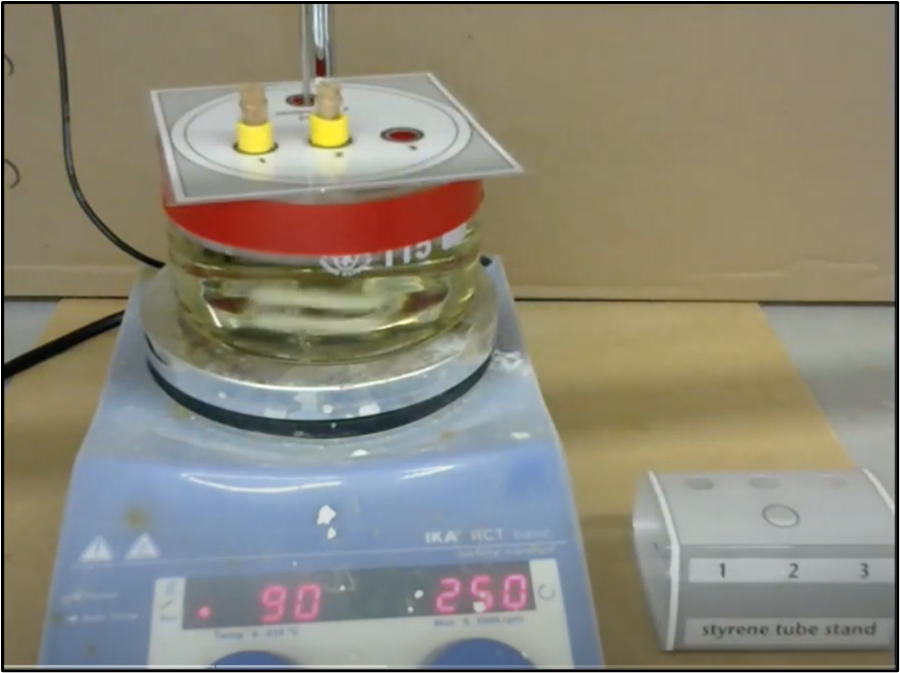
\includegraphics[width=\columnwidth]{images/fig1.png}
    \caption{Screenshot of a video walkthrough adapted with an Audio Description\textsuperscript{81}. Transcript is in the Supplementary Information.}
    \label{Figure 1}
\end{figure}

\subsection*{Sign Language}
For many D/HH individuals, sign language is their first language; and for example in the UK approximately one in a thousand people use British Sign Language as their preferred language. However, D/HH people are almost always expected to have to use close captions at best. Allowing lip reading is encouraged as far as possible. Worldwide there are estimated over 130 sign languages\textsuperscript{82} and probably more than twice that number as even amongst countries that share the same spoken language there are different sign languages, for example American, Australian and British sign languages differ from each other.

\textbf{Chemical Sciences Sign Language:} There is much work still to be done to create a lexicon of chemical sign language\textsuperscript{73,83} and for this to be globally consistent – excellent examples of such an approach have been demonstrated by Quantum ASL\textsuperscript{84} and also by the Scottish Sensory Centre\textsuperscript{85}. The ongoing creation of inclusive digital resources by educators presents the opportunity for these to be accompanied by sign language translations that will help address the underrepresentation of D/HH learners in the chemical sciences\textsuperscript{86} and chemistry educators are strongly encouraged to be more inclusive in this regard. Again, open sharing of recordings that have been translated in to sign language would be a very welcome practice from the chemical community.

\subsection*{Alt Text - Alternative text for all images, including reaction schemes, graphs, spectra and equations.}

Arguably the most challenging aspect of universal design is the alternative text or ‘alt text’ element. Alt text essentially is a description of an image when that image can’t be viewed. As discussed earlier, there is a pervasive and heavy reliance on the visual within the chemical sciences and it may therefore be difficult to rationalise how this barrier can be overcome. For an excellent riposte and a perspective on how, in chemistry, visually impaired individuals can visualise without vision the reader is referred to a review by Wedler and colleagues\textsuperscript{87} highlighting a wide range of methodologies and adaptations that are inclusive of blind and visually impaired individuals. A number of articles by Supalo and co-workers deserve special attention as they highlight how instructors can improve their effectiveness in teaching blind chemistry students\textsuperscript{88–91}.  With respect to alt text, the reader is directed to a first-rate example\textsuperscript{92} of constructing useful descriptions of complex molecular structures from the perspective of a blind chemist. As educational best practice there is no reason why many spectra such as those found in infrared and NMR analysis (see Figure 2 for an example) cannot use the standard written notation used in research articles as the alt text. 

\begin{figure}[htb]
    \centering
    
\includegraphics[width=\columnwidth]{images/fig2.png}
    \caption{Alternative text description: \textsuperscript{13}C NMR of N-(exo-himoyl)-glycinoyl chloride, showing peaks at 39,1; 42.8; 45.4; 48.1; 76.7; 77.1; 77.4; 138.0; 171.7; 177.3 parts per million (ppm). The reference peaks for deuterated chloroform are also visible as a triplet at 77.1ppm}
    \label{Figure 2}
\end{figure}

Chemical structures and equations remain a significant challenge but again it is worth noting that often what is being represented may actually be a small change to a large molecule (e.g. organic functional group interconversion) and so a useful alt text can still be created and indeed organic chemists, when teaching, often use the ‘R-group’ notation to denote parts of the molecule that are not involved in a reaction to avoid visual confusion. Optical character recognition when applied to chemical structures, known as the Chemical Literature Extraction and Aloud-Reading System (CLEARS)\textsuperscript{93} has made great strides in converting graphic structures to chemical names and whilst this is not yet sufficiently accurate to be automated, as this would require a 100\% success rate, it is highly promising. 

\subsection*{Example of universal design practices in a chemistry PowerPoint slide}

\begin{figure*}[htb]
    \centering
    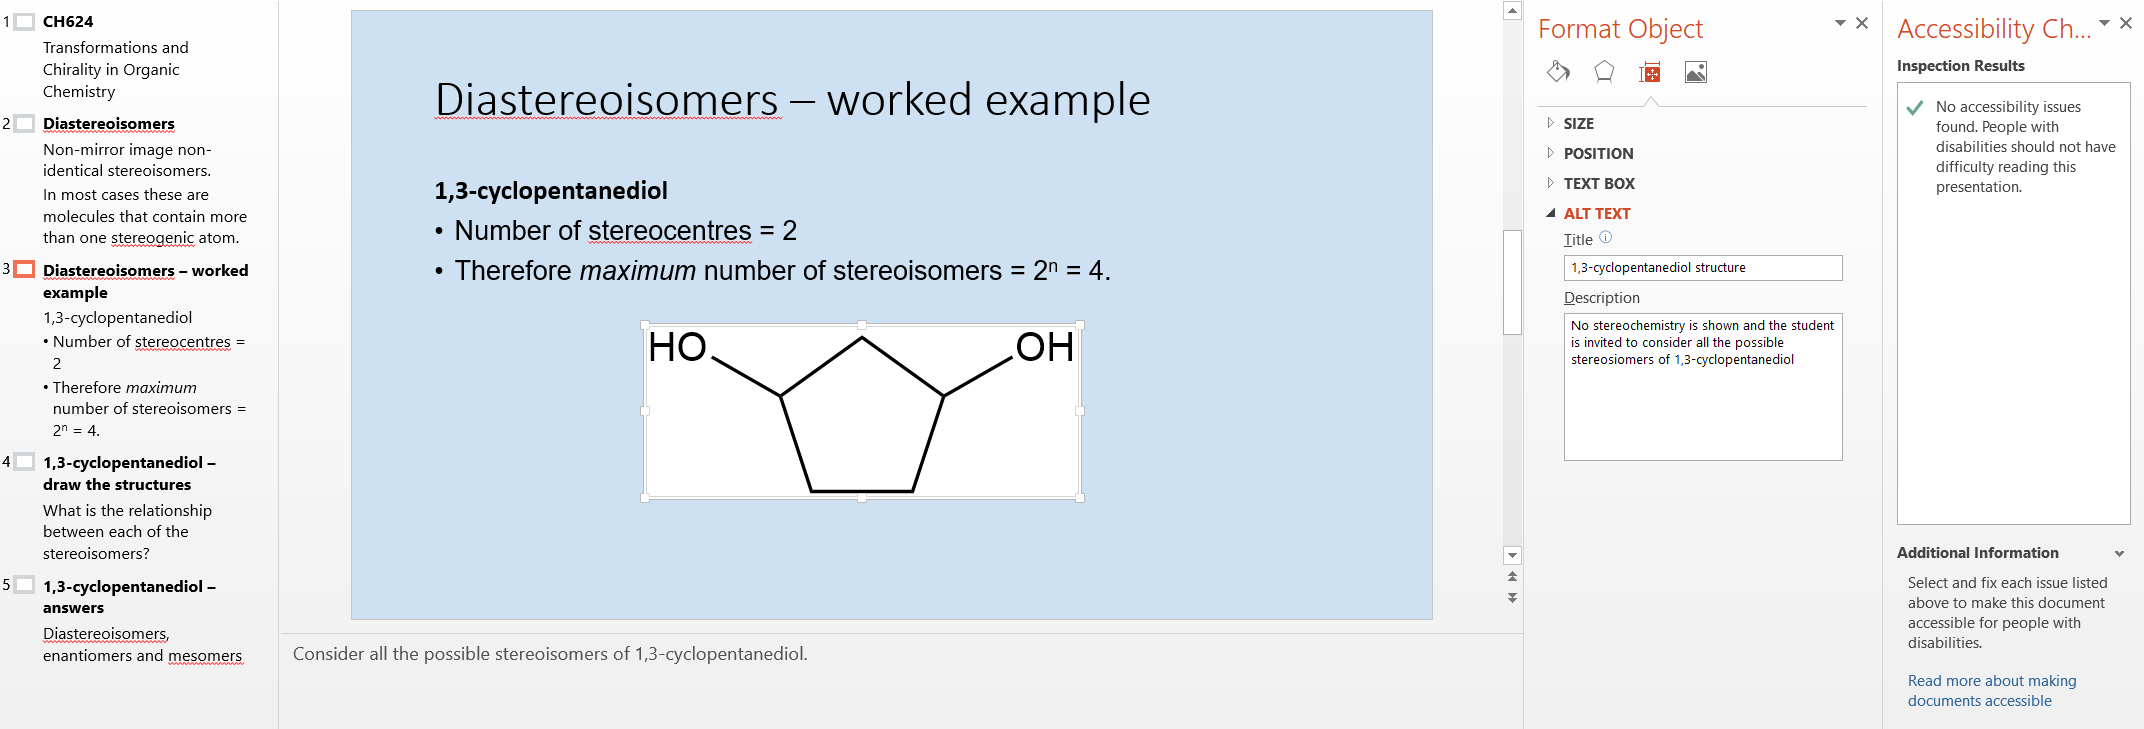
\includegraphics[width=\textwidth]{images/fig3.png}
    \caption{PowerPoint slide highlighting accessibility features}
    \label{Figure 3}
\end{figure*}

In Figure 3, the PowerPoint slide is shown with the navigational view showing a title for each slide in the presentation. This makes it easier to navigate using a keyboard. Each slide has a unique title. The image in the slide has an alternative text description. Whilst the use of the words ‘image’ or ‘picture’ in the title are discouraged as they are superfluous and distracting, the word ‘structure’ may be appropriate as it clarifies the representation of 1,3-cyclopentanediol. The slide itself uses sans serif font of no less than 20 point and the presentation has been checked for accessibility issues using the inbuilt functions. The slide has a plain pastel blue background in keeping with readability best practices, which currently are not checked with the inbuilt functions. The slide is free of distracting logos and background effects. The slide number also has not been included as most people use the navigational section to find a slide. However if the presentation was large and was to be printed then slide numbers may prove useful. A feature that may not be obvious from the image in Figure 2 is that the slide has been prepared selecting an appropriate template such that the reading order is unambiguous, i.e. ‘title’ followed by ‘subtitle’ followed by ‘text’ followed by ‘image’. This is important for people who navigate using keyboards. Additional content can subsequently be added but it is important to manually check that the reading order is correct. The alt text does repeat a point covered in the notes and sometimes this may be difficult to avoid as not all students may access the alt text or the notes. An aspect that may create inaccessibility however is the term ‘2\textsuperscript{n}’ meaning ‘two to the power of n’ which many automated assistive readers will convey linearly as ‘2n’ i.e. ‘two times n’ and this point is discussed below.

\textbf{Mathematical equations:} Conveying mathematical notations to visually impaired people is yet another challenge that has not been satisfactorily solved\textsuperscript{94}. Mathematical notation in Braille for example does not have a global standard, it varies across different countries.  In addition, not all visually impaired students practice Braille and there is evidence that students who do use Braille notation are less likely to participate at higher levels of education\textsuperscript{95}. There is evidence that assistive technology does not yet reduce barriers sufficiently to achieve educational parity between visually impaired and non-visually impaired students, and furthermore visually impaired students tend to perform below their potential ability when compared to other subjects such as social sciences\textsuperscript{96}. Comparison of assistive technologies or approaches is difficult as it is not always clear what the level of assistive technology is and how they serve different educational stages\textsuperscript{95}. What does seem to hold true is that students with visual impairments can be ‘as successful as other students in sciences and mathematics given knowledgeable and supportive teachers’ and furthermore, the ‘adaptations provided benefit the entire class’\textsuperscript{97}. 

There are approaches to convey mathematical equations linearly for example by conversion to LateX but these require a level of learning the coding language from the students and the resulting expressions can be very cumbersome\textsuperscript{98}. The other problem with LateX documents is that these are not accessible to automated readers. The requirements for textbooks to improve their mathematical accessibility has been eloquently argued\textsuperscript{99} and is reflective of the challenges faced in the sciences in general including chemistry to provide inclusive description for non-word material. The solution which is currently just out of reach is for automated readers to describe equations linearly using unencumbered coding methods. This would also require reading the secondary graphics often used in mathematics (for example strikethrough lines when fractions are simplified) and be based on a good understanding of how people actually read mathematical equations in order to interpret them\textsuperscript{94}. In the absence of such technology being mainstream and readily available, educators should consider providing alternatives such as voice recordings describing equations linearly, with the associated transcripts.

\subsection*{Websites}
When creating website and webpages international guidelines relating to digital accessibility should be adhered to, and in many countries these are now a legal requirement for public bodies\textsuperscript{100}. However, compliance does not automatically result in usability.  For example learning management systems such as Moodle are also considered as websites and the organisational and navigational structure can affect how easy or otherwise they are to navigate to retrieve teaching content even if compliant. 

Key aspects that should be regularly reviewed include

\begin{itemize}
    \item Fully navigable without using a mouse, i.e. using a keyboard or voice recognition tool. In practice many users do not know how to navigate without a mouse and therefore to check for compliance. 
    \item Ensuring a good organisational structure particularly for learning management systems - that is repeated systematically across modules - will facilitate navigation for all users.
    \item Able to be magnified up to 200\% without losing text from the screen. A note of caution. As stated previously, whilst magnification helps – for some users who have good acuity but it is restricted to a small area only, a larger size will lose the context of the image or text, so for example they would have to read text one letter at the time when they could read the same text one word at the time. 
    \item All text and images to be read in the correct sequence by a screen reader.
    \item Any hyperlinks to be readable and self-evident without automatically hyperlinking unless selected.
    \item Any documents to be digitally accessible.
    \item Any audio-visual information to be close captioned and/or a transcription provided
    \item All teaching material to be available at least 24h before a class but ideally from the start of term.
\end{itemize}

From the perspective of a chemistry educator it is invaluable if the teaching materials can be supplemented by electronic textbooks which can provide a valuable alternative format for the topics being covered, in which case lectures should be carefully mapped to the textbook. Some publishers are now supplying material with good quality alt text for the imagery which is available to use for educational purposes and academics are encouraged to support these best practices from publishers, and insist that their institutions adopt textbooks which have digitally accessible versions.

A periodic table has been created by the American Chemical Society (ACS) which is keyboard compatible and can be read by assistive readers\textsuperscript{101}. The Royal Society of Chemistry (RSC) has a periodic table which includes podcasts with transcripts and videos with corrected close caption\-ing\textsuperscript{102}. Both of these periodic tables, as well as other periodic tables designed for accessibility by blind people\textsuperscript{103} are freely available valuable resources that do not need to be duplicated by others and underline the fact that a range of resources may be required to provide breadth of inclusivity and usability.

\subsection*{Summary and solving the disproportionate burden problem}

As discussed, achieving compliance with digital accessibility regulations, means that a number of criteria need to be addressed, some of which require significant additional resources in either time or other costs to achieve. This has led to some organisations claiming that meeting these resource costs to achieve compliance is too detrimentally impactful and creates what has been termed\textsuperscript{104} a ‘disproportionate burden’.  For chemistry educators who create teaching materials these fall into the following main practical issues:

\begin{itemize}
    \item Correct close captioning, audio descriptions and transcripts for all video and recorded material
    \item Sign language
    \item Alternative text for all images, including reaction schemes, graphs, spectra and equations
    \item Mathematical equations
\end{itemize}

The best way that this disproportionate burden can be overcome is if institutes and organisations make freely available their resources and materials. As we have seen in the previous section examples of accessible periodic tables are freely available\textsuperscript{101–103} but each of these would have taken considerable time and care to construct, and each caters to a slightly different audience. Broadly speaking most universities will have a great overlap of topics and it should be possible therefore to ‘borrow’ and ‘lend’ to each other with respect to resources that have been specially prepared for greater inclusivity.  A greater awareness of accessibility requirements and training of people in good practices is also required. As an example, the next section outlines the outcome of training student cohorts to embed digital accessibility in their work.

\section*{CASE STUDY: STUDENT TRAINING AND DEVELOPMENT}
Three separate cohorts of students at the University of Kent enrolled on Chemistry or Forensic Science degree programmes were given training in universal design best practices relating to PowerPoint and asked to incorporate these in their presentations. The requirement to include these best practices was not mandatory and no marks were associated.  

The training session itself was light touch and consisted in a 20 minute presentation on how to prepare PowerPoint slides where the following was emphasized: 

\begin{enumerate}
    \item Keep a simple uncluttered layout - as this is less visually distracting and less time needs to be spent trying to distinguish information from background design
    \item Use standard templates with software generated title headings – this helps a reader to quickly search or ‘navigate’ through the slides and ensures the correct reading order
    \item Each slide to have a unique title – again this helps with the navigation of the presentation, and ideally no two slides should have the same name
    \item Use 24 point font minimum and use sans-serif font – to aid readability
    \item Choose suitable colour contrasts – this again is related to readability and it can be linked if appropriate to a further consideration of ensuring that information is not contained in colour alone 
    \item Use web links that say what they are – this prevents someone having to click a link to find out if it important or can be ignored
    \item Provide alternative text for images – assume that the user can’t see the image. Alt text should explain the same information that the presenter is wishing to convey
\end{enumerate}

\textbf{Student take up:} The take up was excellent and from a total number of seventyone students all but one student engaged with at least one aspect of best practice – students recognizing the value of the employability skills gained. Students in the main addressed the following usability best practice criteria: navigational preparation of their documents, appropriate colour contrast and font size (Table 1). Automated accessibility checkers were used to evaluate the student submissions. Blackboard Ally is used at the University of Kent and checks for colour contrast, images with alt text, tables without headings and documents without titles, and produces a percentage accessibility score range of low (0-33\%); medium (33-67\%) and high (67-100\%). The result was that the students’ documents scored well on Blackboard Ally with a high average percentage score. As a note of caution in using Blackboard Ally scores, these can be used to give an indication but should not be relied upon for a meaningful score as the checker produces a score based on the number of errors not the type of errors. The submissions were also individually examined by the author using the in-built Microsoft accessibility checker (key checks include navigational layout of documents, alt text, tables without headers and PowerPoint reading order) which however does not provide a score. Finally font size was checked manually as neither of the automated accessibility checkers has font size as a criterium. In order to provide a meaningful comparison, results from previous a cohort that had not received accessibility training were also analyzed. The untrained subsets submitted presentations which received a medium Blackboard Ally score, and there were other faults also picked up by the Microsoft checker. Of the two submissions that scored well, one was because no images had been included, whereas the other submission the student was already knowledgeable in constructing slides with good navigability and had applied good practice as standard, which was positive to note. In summary, the cohort who did receive training significantly improved the average accessibility profile for their submissions (Figure 4). 

\begin{figure*}[htb]
    \centering
    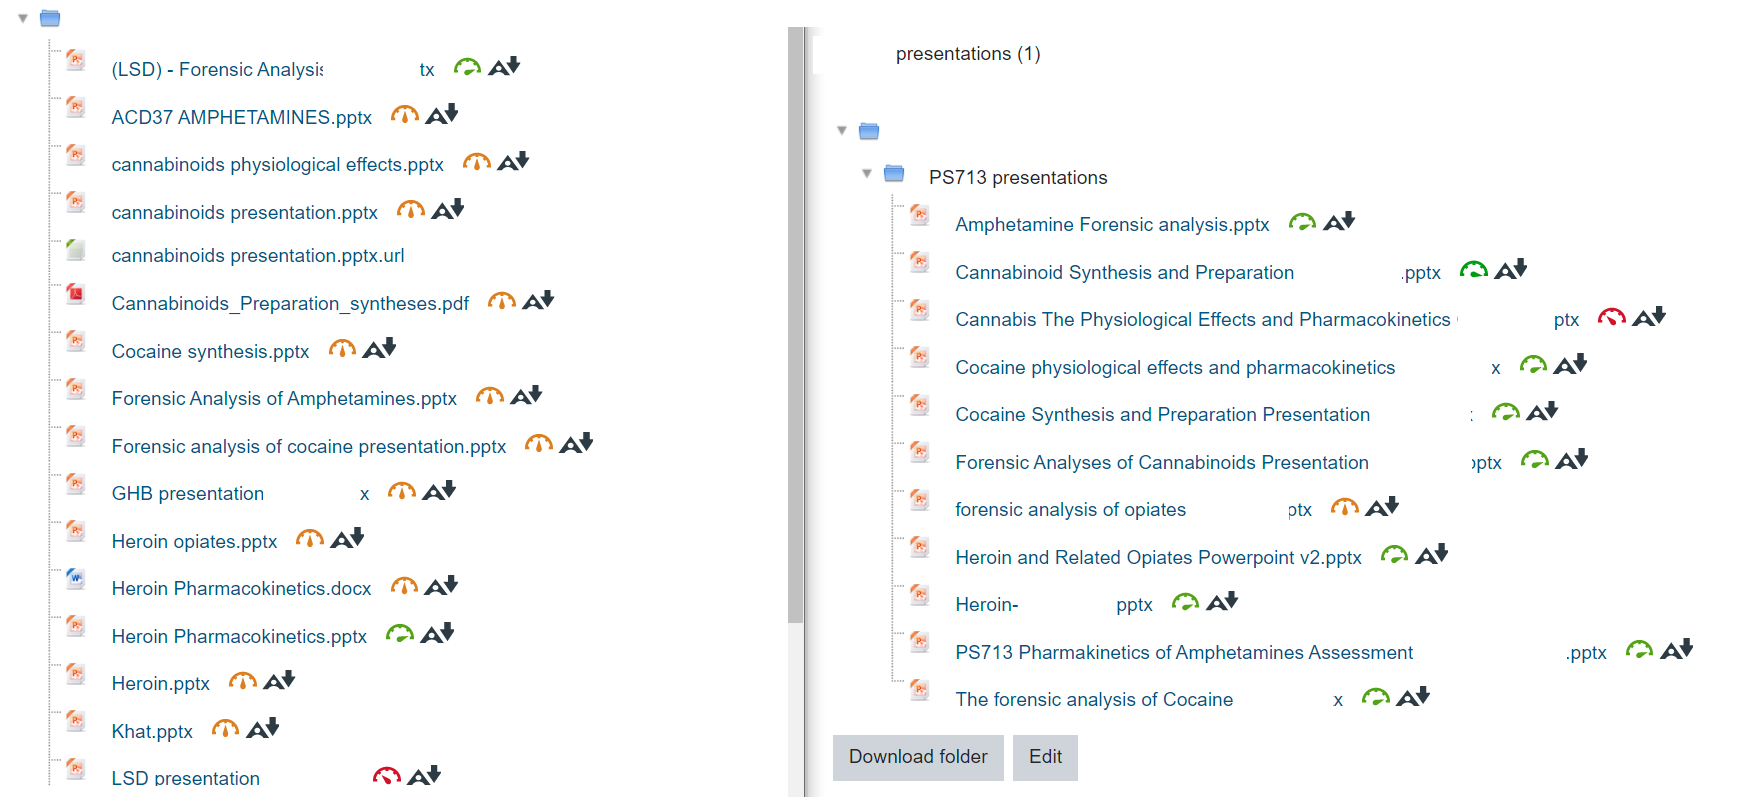
\includegraphics[width=\textwidth]{images/fig4.png}
    \caption{Comparison of cohorts pre- and post-training on universal design practices: On the left a screenshot of a Moodle submission page from an untrained cohort and on the right a cohort that have received training. (Dates and names deleted). The score dials from the screenshot on the right also point to the right and are colour coded green to signify that they are acceptable, rather than amber or red which populate the majority of the scores from the untrained cohort.}
    \label{Figure 4}
\end{figure*}

In respect to the note of caution in using Blackboard Ally scores,  in the cohort of students who had been trained on universal design, there was one submission that scored poorly because the background contrast was poor throughout, even though the navigability was good and the font was sans serif and no less than 20 point. A simple change of background would have raised the score to very good. It should be noted that students did not have access to Blackboard Ally (this is available for staff only) but were trained to use the Microsoft accessibility checker, which currently does not pick up on luminescence contrast. Neither the Blackboard Ally or Microsoft systems check for font size, this was done manually.

\begin{table*}[th]
\caption{Summary of student engagement with universal design criteria}
\begin{tabular}{|l|l|l|l|}
\hline
\textbf{Universal Design criteria} & \textbf{Additional time required as a percentage of preparation time} & \textbf{Number of students engaging with the criteria out of 71 total} & \textbf{Engagement as a percentage of overall student numbers} \\ \hline
Navigability & Low <5\% & 70 & 99\% \\ \hline
Large font & Low <5\% & 64 & 90\% \\ \hline
Colour contrast & Low <5\% & 59 & 83\% \\ \hline
Alternative text & High 20-80\% & 9 & 13\% \\ \hline
\end{tabular}
\end{table*}

Alternative text adjustments were in the main not addressed by students (Table 1), with only a handful of exceptions across all the cohorts. This reflects the discussion in the previous section that alternative text provision is one area where students from the chemical sciences face a discipline difficulty and indeed it can be difficult at times to provide meaningful alt text for complex structures or visual representations.  One student who did engage with the alt text stated that for her 15 min presentation (thirteen slides) it probably added over 30 min of preparation time but that she did it as she went along and found the process useful as it made her focus on the value of what was being included; a screenshot is shown in Figure 5 and the presentation returned as perfect on both Microsoft and Blackboard Ally accessibility checkers.

\begin{figure*}[htb]
    \centering
    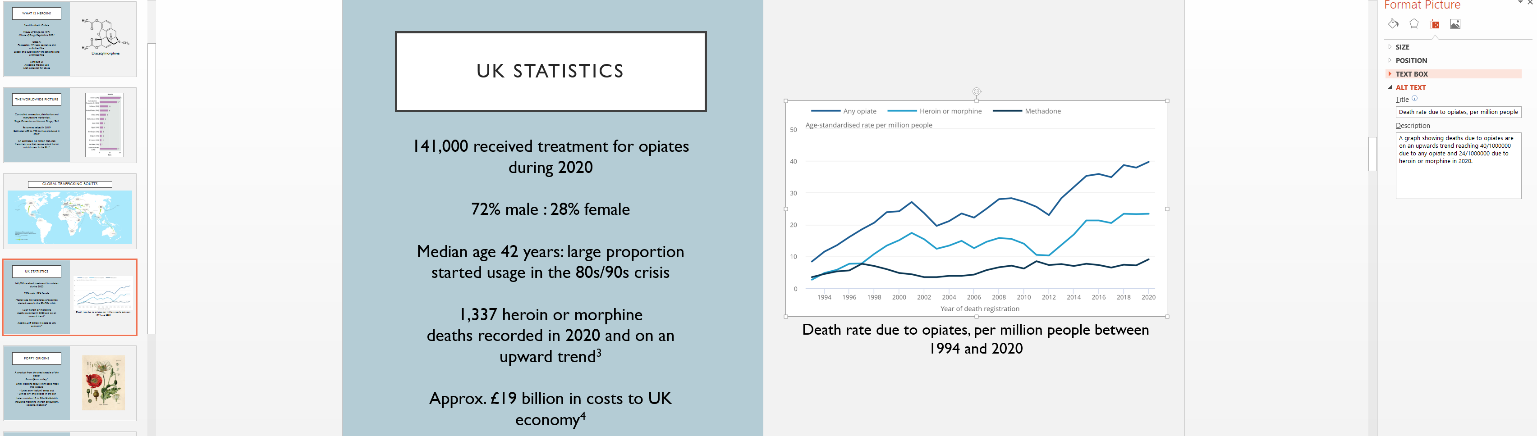
\includegraphics[width=\textwidth]{images/fig5.png}
    \caption{A PowerPoint slide prepared by a student using digital accessibility best practices.}
    \label{Figure 5}
\end{figure*}

This case study of training the students underlined the fact that many adjustments are easy to make and are perceived as valuable. The feedback from the students was overwhelmingly positive: \textit{This is useful knowledge for after we graduate; It is so important; It makes it clearer and easier to follow, why would anybody not do this?…} Feedback from a graduate:  I am grateful and happy that I am using it [at work] and I only learnt about it through your project; it really does help\textsuperscript{105}.

\section*{SPECIFIC LABORATORY SUPPORT}

As outlined in the introduction, the last part of inclusive chemistry education involves practical work. Computers are not typically associated with organic or inorganic wet lab environments, however they can form an integral part of assisting visually impaired students. 

\begin{figure}[htbp]
    \centering
    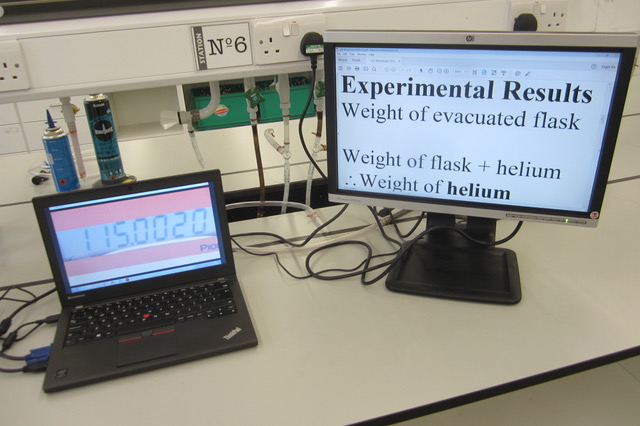
\includegraphics[width=0.95\columnwidth]{images/fig6.png}
    \caption{One screen is a digital readout from a weighing scale that has been captured by a webcam and magnified. The other screen shows an excerpt from the lab manual that the student is following. The text has been magnified and the student has chosen the desired contrast but the text can also be read automatedly. The student can also input notes using a keyboard if desired. Adapted from reference 19.}
    \label{Figure 6}
\end{figure}

A set-up as shown in Figure 6 was used at our institute, and allowed for a visually impaired student to readily access lab manuals, notebooks and other information which had been prepared using digital accessibility universal design features and enabled the student to attend and complete undergraduate laboratory classes.

Bespoke adaptations were made using web-cams which enabled the student to use his residual vision to safely perform and follow a reaction. The example shown here is a titration (Figures 6-12). The student’s residual vision was limited to a small area in one eye only, and only if the object or screen or paper is placed very close to the eye. The adaptations shown are relatively low cost and non-specialized. The student had access to a PhD chemistry level assistant who could report observations if requested and could assist with locating equipment or reagents but was careful not to perform the experiment for the student. The laboratory area required was roughly twice that of a sighted student. Technical staff and instructors were briefed on how to engage with a blind person\textsuperscript{106}.

\begin{figure}[htbp]
    \centering
    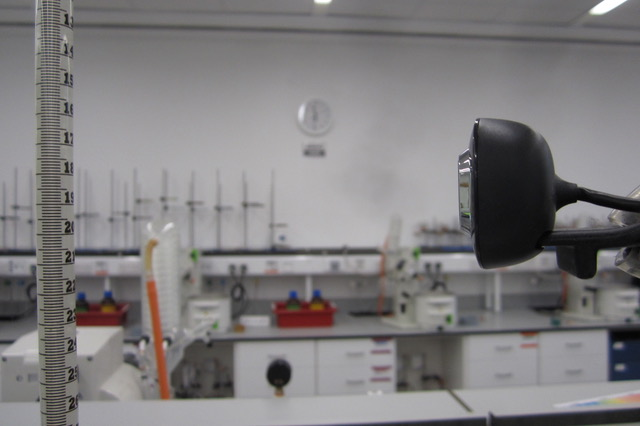
\includegraphics[width=0.95\columnwidth]{images/fig7.jpeg}
    \caption{Using webcams to enhance visual feedback. A webcam is clamped on a retort stand such that it can view a burette. The webcam image will be magnified on to a screen (not shown in the image) such that it will allow a student with visual impairment to better see the start and end points of the titration. Also, the burette, which is clamped to a retort stand, is placed inside a large spill tray.}
    \label{Figure 7}
\end{figure}

\begin{figure}[htbp]
    \centering
    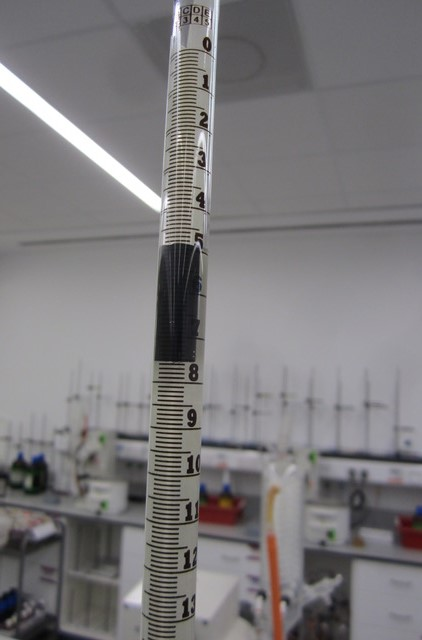
\includegraphics[width=\columnwidth]{images/fig8.jpeg}
    \caption{Contrast on the burette. The burette has black tape applied in the critical area where a reading will occur. This is to allow for better visual contrast between the tape and meniscus of the solution.}
    \label{Figure 8}
\end{figure}

\begin{figure}[htbp]
    \centering
    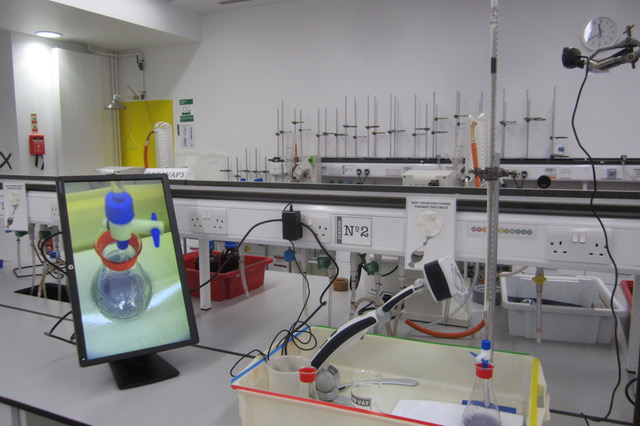
\includegraphics[width=\columnwidth]{images/fig9.jpeg}
    \caption{End-point visualization. A webcam is focused on the burette, set-up inside a splash tray, to visualise the burette reading. A separate webcam is focused on the titre flask to observe the endpoint. To the left of the splash tray is a screen showing the titre flask magnified for better visualisation. This also means that the student does not have to get close to the chemicals in the flask.}
    \label{Figure 9}
\end{figure}

\begin{figure}[htbp]
    \centering
    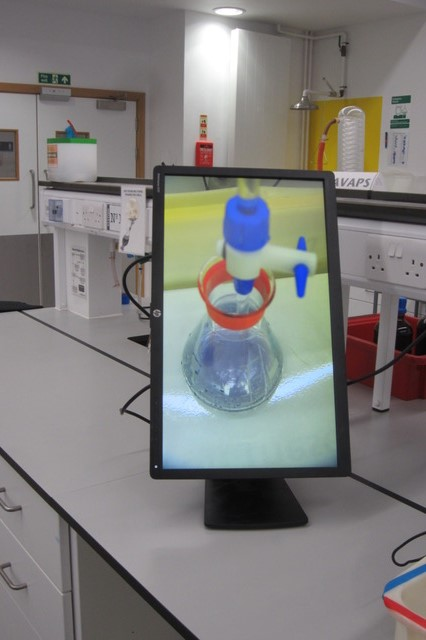
\includegraphics[width=\columnwidth]{images/fig10a.jpeg}
    \caption{Webcam display. Image of the titre flask captured by a webcam and displayed on a screen allowing the student to observe the endpoint of the reaction without needing to get close to the flask and chemicals.}
    \label{Figure 10}
\end{figure}

\begin{figure}[htbp]
    \centering
    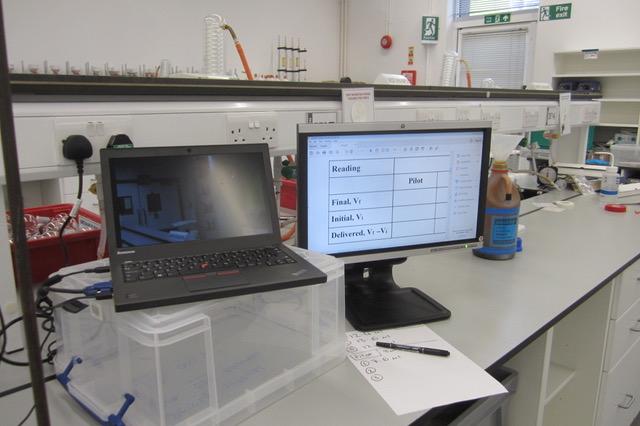
\includegraphics[width=\columnwidth]{images/fig11.jpeg}
    \caption{Notebook input. The image shows a laptop connected to a larger display screen. This makes it easier for the student to input data.}
    \label{Figure 11}
\end{figure}

\begin{figure}[htbp]
    \centering
    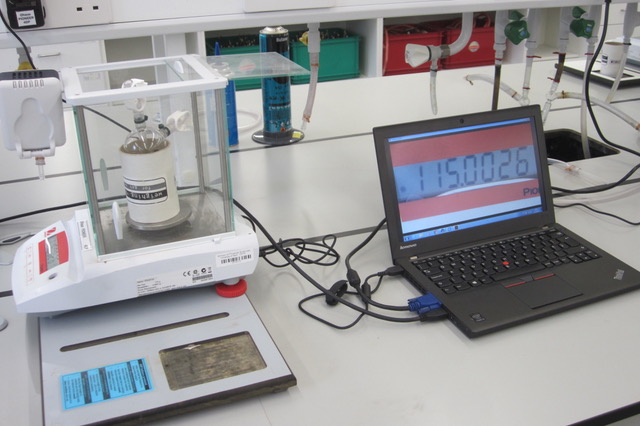
\includegraphics[width=\columnwidth]{images/fig12.jpeg}
    \caption{Magnifying readings. Image shows how the digital readout of a weighing scale can be captured by a webcam and displayed on a laptop with the image magnified to improve its readability. It also allows a student to get close to the screen without impediment, to better read the digits.}
    \label{Figure 12}
\end{figure}

\section*{CONCLUSIONS}
The advancement of digital teaching resources and associated pedagogies has been shown to contribute positively to education but it has bought its own challenges and failings with respect to inclusivity and accessibility, particularly for the chemical sciences. Meeting these challenges however results in universal design good practices which bring advantages to all learners and to educationalists.  There are significant challenges for chemical science educators in that the subject is heavily reliant on the visual and there are no simple automated solutions for providing alternative formats to the complex range of visual information, including mathematical notation. There is no standard sign language for chemical lexicons, which does however represent an opportunity for the community to develop an internationally agreed chemical sign language. Students are receptive to both training and engagement in universal design practices but take up on providing alternative text remained low. Finally, this article is a call to arms asking that material that is created in-house by chemistry educators worldwide, whether it be videos, spectra, graphs, etc., can be made publicly available such that over time it will offer full coverage of chemistry topics. We share here an example of how webcams can be used to include a visually impaired student in a laboratory practical.

\section*{ASSOCIATED CONTENT}
\textit{Audio description transcript for reference 81 is provided after the references}

\section*{ACKNOWLEDGMENTS}
The Author is grateful to Beatrix Biagini, Dr Charlotte Harris and Ben Watson for helpful discussions, advice and inspiration. Dr Alexander Wright and Nic Duncan for assistance in creating the audio description video cited in reference 81. The students on Chemistry and Forensic Science CH620 and PS713/PSCI7130 modules at Kent for engaging with accessibility best practices. In particular I would like to thank the following students: William Housden, Sabaa Hussain and Eleanor Sutherland for invaluable engagement and feedback on some of the accessibility practices discussed in this article and for granting permission to use their work. Figures 6-12 Spartaco Landi and Philip Marsh for laboratory set-up and photography. The Royal Society of Chemistry EDI section for support including conferences, networking and helpful discussions.

\end{large}
\clearpage
\section*{REFERENCES}\par 

\leftskip 0.25in
\parindent -0.25in % create hanging indents for references. if article has content after references, set leftskip and parindent to 0

(1)	\textit{Home | Web Accessibility Initiative (WAI) | W3C}. \url{https://www.w3.org/WAI/} (accessed 2021-06-23).

(2)	UE. The European Disability Strategy 2010-2020 - Summary. \textit{Eur. Comm}. \textbf{2010}, 1–12.

(3)	\textit{The Economic Impact of Sight Loss and Blindness in the UK Adult Population, 2013 Royal National Institute of Blind People (RNIB) Economic Impact of Sight Loss and Blindness in the UK}; 2014. \url{www.deloitte.com/au/about} (accessed 2021-06-29).

(4)	Bodner, G. M.; Domin, D. S. Mental Models: The Role of Representations in Problem Solving in Chemistry PROCEEDINGS Introduction to Research on Problem Solving in Chemistry. \textit{Univ. Chem. Educ}. \textbf{2000}, \textit{4} (1), 24–30.

(5)	Popova, M.; Jones, T. Chemistry Instructors’ Intentions toward Developing, Teaching, and Assessing Student Representational Competence Skills. \textit{Chem. Educ. Res. Pract}. \textbf{2021}, \textit{22} (3), 733–748. \url{https://doi.org/10.1039/D0RP00329H}.

(6)	Ramnarain, U.; Joseph, A. Learning Difficulties Experienced by Grade 12 South African Students in the Chemical Representation of Phenomena. \textit{Chem. Educ. Res. Pract}. \textbf{2012}, \textit{13} (4), 462–470. \url{https://doi.org/10.1039/c2rp20071f}.

(7)	Kozma, R. B.; Russell, J. \textit{Multimedia and Understanding: Expert and Novice Responses to Different Representations of Chemical Phenomena}; 1997; Vol. 34, pp 949–968.

(8)	Cooper, M. M.; Grove, N.; Underwood, S. M.; Klymkowsky, M. W. Lost in Lewis Structures: An Investigation of Student Difficulties in Developing Representational Competence. \textit{J. Chem. Educ}. \textbf{2009}, \textit{87} (8). \url{https://doi.org/10.1021/ed900004y}.

(9)	Brown, E. The Fight for Accessibility. \textit{Nature} \textbf{2016}, \textit{532} (7597), 137–139. \url{https://doi.org/10.1038/NJ7597-137A}.

(10)	\textit{Accessible science education | Feature | Chemistry World}. \url{https://www.chemistryworld.com/features/accessible-science-education/3010431.article} (accessed 2021-06-30).

(11)	Royal Society of Chemistry. \textit{Diversity Data Report 2020}; 2020. \url{www.rsc.org} (accessed 2021-06-30).

(12)	\textit{What are HE students’ progression rates and qualifications?: Personal characteristics | HESA}. \url{https://www.hesa.ac.uk/data-and-analysis/students/outcomes/characteristics} (accessed 2021-07-01).

(13)	\textit{Disability and employment, UK - Office for National Statistics}. 
\url{https://www.ons.gov.uk/peoplepopulationandcommunity/healthandsocialcare/disability/bulletins/disabilityandemploymentuk/2019#measuring-the-data} (accessed 2021-07-01).

(14)	Royal Society of Chemistry. Diversity Landscape of the Chemical Sciences A Report by the Royal Society of Chemistry. \textbf{2018}, 18.

(15)	Cumberland, P. M.; Pathai, S.; Rahi, J. S. Prevalence of Eye Disease in Early Childhood and Associated Factors: Findings from the Millennium Cohort Study. \textit{Ophthalmology} \textbf{2010}, \textit{117} (11), 2184-2190.e3. \url{https://doi.org/10.1016/j.ophtha.2010.03.004}.

(16)	Jack.org. Jack.Org Annual Report: Fiscal Year 2019. \textbf{2019}.

(17)	\textit{Why do billions of people still not have glasses? - BBC News}. \url{https://www.bbc.co.uk/news/business-49991877} (accessed 2021-06-23).

(18)	Smith ECW; Congdon, N; Frick, K.; Kassalow, J.; Naidoo, K.; Sloan, J. A. \textit{Eyeglasses for Global Development: Bridging the Visual Divide - Vision Impact Institute}. \url{https://visionimpactinstitute.org/research/eyeglasses-global-development-bridging-visual-divide/} (accessed 2021-06-23).

(19)	Biagini, S. C. G., Duncan, N., Watson, B. \textit{Including blind and visually impaired students in the chemical sciences: establishing good practices RSC Inclusion and Diversity Forum 2020}. \url{https://kar.kent.ac.uk/84837/}

(20)	\textit{All WAI Translations | Web Accessibility Initiative (WAI) | W3C}. \url{https://www.w3.org/WAI/translations/} (accessed 2022-04-14).

(21)	ETSI; CENELEC; \& CEN. EN 301 459 v2.1.2 (2018-08): \textit{Accessibility Requirements for ICT Products and Services}; 2018.

(22)	Office for National Statistics. Exploring the UK’s Digital Divide - Office for National Statistics. \textit{Off. Natl. Stat}. \textbf{2019}, 1–24.

(23)	Bryan, A. H. Chemistry for the Blind. \textit{Sci. Educ}. \textbf{1952}, \textit{36} (2), 91–95. \url{https://doi.org/10.1002/sce.3730360208}.

(24)	Boyd-Kimball, D. Adaptive Instructional Aids for Teaching a Blind Student in a Nonmajors College Chemistry Course. \textit{J. Chem. Educ}. \textbf{2012}, \textit{89} (11), 1395–1399. \url{https://doi.org/10.1021/ed1000153}.

(25)	Pereira, F.; Ponte-E-Sousa, J. C.; Fartaria, R. P. S.; Bonifácio, V. D. B.; Mata, P.; Aires-De-Sousa, J.; Lobo, A. M. Sonified Infrared Spectra and Their Interpretation by Blind and Visually Impaired Students. \textit{J. Chem. Educ}. \textbf{2013}, \textit{90} (8), 1028–1031. \url{https://doi.org/10.1021/ed4000124}.

(26)	Pereira, F.; Aires-De-Sousa, J.; Bonifácio, V. D. B.; Mata, P.; Lobo, A. M. MOLinsight: A Web Portal for the Processing of Molecular Structures by Blind Students. \textit{J. Chem. Educ}. \textbf{2011}, \textit{88} (3), 361–362. \url{https://doi.org/10.1021/ed100723v}.

(27)	Harshman, J.; Bretz, S. L.; Yezierski, E. Seeing Chemistry through the Eyes of the Blind: A Case Study Examining Multiple Gas Law Representations. \textit{J. Chem. Educ}. \textbf{2013}, \textit{90} (6), 710–716. \url{https://doi.org/10.1021/ed3005903}.

(28)	Anderson, J. L. Chemical Instrumentation for the Visually Handicapped. \textit{J. Chem. Educ}. \textbf{1982}, \textit{59} (10), 871–872. \url{https://doi.org/10.1021/ed059p871}.

(29)	Lunney, D.; Morrison, R. C. High Technology Laboratory Aids for Visually Handicapped Chemistry Students. \textit{J. Chem. Educ}. \textbf{1981}, \textit{58} (3), 228–231. \url{https://doi.org/10.1021/ed058p228}.

(30)	Clauss, A. JCE Concept Connections: Making Chemistry Accessible. \textit{J. Chem. Educ}. \textbf{2009}, \textit{86} (5), 591. \url{https://doi.org/10.1021/ed086p591}.

(31)	Tallman, D. E. A pH Titration Apparatus for the Blind Student. \textit{J. Chem. Educ}. \textbf{1978}, \textit{55} (9), 605–606. \url{https://doi.org/10.1021/ed055p605}.

(32)	Hiemenz, P. C.; Pfeiffer, E. A General Chemistry Experiment for the Blind. \textit{J. Chem. Educ}. \textbf{1972}, \textit{49} (4), 263–265. \url{https://doi.org/10.1021/ed049p263}.

(33)	Ratliff, J. L. Chemistry for the Visually Impaired. \textit{J. Chem. Educ}. \textbf{1997}, \textit{74} (6), 710–711. \url{https://doi.org/10.1021/ed074p710}.

(34)	Wedler, H. B.; Cohen, S. R.; Davis, R. L.; Harrison, J. G.; Siebert, M. R.; Willenbring, D.; Hamann, C. S.; Shaw, J. T.; Tantillo, D. J. Applied Computational Chemistry for the Blind and Visually Impaired. \textit{J. Chem. Educ}. \textbf{2012}, \textit{89} (11), 1400–1404. \url{https://doi.org/10.1021/ed3000364}.

(35)	Tombaugh, D. Chemistry and the Visually Impaired: Available Teaching Aids. \textit{J. Chem. Educ}. \textbf{1981}, \textit{58} (3), 222–226. \url{https://doi.org/10.1021/ed058p222}.

(36)	Miner, D. L.; Nieman, E.; Ron, E.; Swanson, A. B.; Woods, E.;; Michael, E. \textit{Teaching Chemistry to Students with Disabilities: A Manual for High Schools, Colleges, and Graduate Programs. 4th}; 2001.

(37)	Poon, T.; Ovadia, R. Using Tactile Learning Aids for Sudents with Visual Impairments in a First-Semester Organic Chemistry Course. \textit{J. Chem. Educ}. \textbf{2008}, \textit{85} (2), 240–242. \url{https://doi.org/10.1021/ed085p240}.

(38)	Wedler, H. B.; Boyes, L.; Davis, R. L.; Flynn, D.; Franz, A.; Hamann, C. S.; Harrison, J. G.; Lodewyk, M. W.; Milinkevich, K. A.; Shaw, J. T.; Tantillo, D. J.; Wang, S. C. Nobody Can See Atoms: Science Camps Highlighting Approaches for Making Chemistry Accessible to Blind and Visually Impaired Students.\textit{ J. Chem. Educ}. \textbf{2014}, \textit{91} (2), 188–194. \url{https://doi.org/10.1021/ed300600p}.

(39)	Ashley Neybert. Perspective from Grad School: When You Are Blind and in Grad School. \textit{CEN Glob. Enterp}. \textbf{2018}, \textit{96} (36), 30–30. \url{https://doi.org/10.1021/cen-09636-cover9}.

(40)	Miecznikowski, J. R.; Guberman-Pfeffer, M. J.; Butrick, E. E.; Colangelo, J. A.; Donaruma, C. E. Adapting Advanced Inorganic Chemistry Lecture and Laboratory Instruction for a Legally Blind Student. \textit{J. Chem. Educ}. \textbf{2015}, \textit{92} (8), 1344–1352. \url{https://doi.org/10.1021/ed500489c}.

(41)	Casas, L.; Estop, E. Virtual and Printed 3D Models for Teaching Crystal Symmetry and Point Groups. \textit{J. Chem. Educ}. \textbf{2015}, \textit{92} (8), 1338–1343. \url{https://doi.org/10.1021/ACS.JCHEMED.5B00147}.

(42)	Rashid, I.; Chehadeh, D. Adaptation of Chemistry Experiments for Middle School Blind or Visually Impaired Students. \textit{J. Chem. Educ}. \textbf{2023}, \textit{100} (6), 2262–2268. \url{https://doi.org/10.1021/acs.jchemed.3c00016}.

(43)	Njardarson, J. T. Introductory Organic Chemistry (First-Semester) for Blind and Visually Impaired Students: Practical Lessons and Experiences. \textit{J. Chem. Educ}. \textbf{2023}, \textit{100} (10), 3960–3967. \url{https://doi.org/10.1021/acs.jchemed.3c00616}.

(44)	Vitoriano, F. A.; Teles, V. L. G.; Rizzatti, I. M.; De Lima, R. C. P. Promoting Inclusive Chemistry Teaching by Developing an Accessible Thermometer for Students with Visual Disabilities. \textit{J. Chem. Educ}. \textbf{2016}, \textit{93} (12), 2046–2051. \url{https://doi.org/10.1021/ACS.JCHEMED.6B00162}.

(45)	Bandyopadhyay, S.; Rathod, B. B. The Sound and Feel of Titrations: A Smartphone Aid for Color-Blind and Visually Impaired Students.  \textit{J. Chem. Educ}. \textbf{2017}. \textit{94} (7), 946-949 \url{https://doi.org/10.1021/acs.jchemed.7b00027}.

(46)	Neely, M. B. Using Technology and Other Assistive Strategies To Aid Students with Disabilities in Performing Chemistry Lab Tasks. \textit{J. Chem. Educ}. \textbf{2007}, \textit{84} (10), 1697. \url{https://doi.org/10.1021/ed084p1697}.

(47)	Supalo, C. A.; Kennedy, S. H. Using Commercially Available Techniques To Make Organic Chemistry Representations Tactile and More Accessible to Students with Blindness or Low Vision. \textit{J. Chem. Educ}. \textbf{2014}, \textit{91} (10), 1745–1747. \url{https://doi.org/10.1021/ed4005936}.

(48)	Nepomuceno, G. M.; Decker, D. M.; Shaw, J. D.; Boyes, L.; Tantillo, D. J.; Wedler, H. B. The Value of Safety and Practicality: Recommendations for Training Disabled Students in the Sciences with a Focus on Blind and Visually Impaired Students in Chemistry Laboratories. \textit{J. Chem. Health Saf}. \textbf{2016}, \textit{23} (1), 5–11. \url{https://doi.org/10.1016/J.JCHAS.2015.02.003}.

(49)	Ali, Z. A.; Rashid, I.; Al-Merri, S. H.; Erjaib, N. A.; Chehadeh, D. Science Camp for Middle School Blind and Visually Impaired Students. \textit{J. Chem. Educ}. \textbf{2024}, \textit{101} (3), 1078–1085. \url{https://doi.org/10.1021/acs.jchemed.3c01122}.

(50)	Khan, M. A. H.; Harrison, T. G.; Wajrak, M.; Grimshaw, M.; Schofield, K. G.; Trew, A. J.; Johal, K.; Morgan, J.; Shallcross, Karen. L.; Sewry, J. D.; Davies-Coleman, M. T.; Shallcross, D. E. Flipping the Thinking on Equality, Diversity, and Inclusion. Why EDI Is Essential for the Development and Progression of the Chemical Sciences: A Case Study Approach. \textit{J. Chem. Educ}. \textbf{2023}, \textit{100} (11), 4279–4286. \url{https://doi.org/10.1021/acs.jchemed.3c00364}.

(51)	Singhal, I.; Balaji, B. S. Open-Source, Tactile 3D Printed Interlockable Tiles Incorporating Valency, Bonding, and Hybridization for Molecular Representation for Sighted and Visually Impaired Students. \textit{J. Chem. Educ}. \textbf{2022}, \textit{99} (4), 1708–1714. \url{https://doi.org/10.1021/acs.jchemed.1c01278}.

(52)	Fernández, G. A.; Ocampo, R. A.; Costantino, A. R.; Dop, N. S. Application of Didactic Strategies as Multisensory Teaching Tools in Organic Chemistry Practices for Students with Visual Disabilities. \textit{J. Chem. Educ}. \textbf{2019}, \textit{96} (4), 691–696. \url{https://doi.org/10.1021/acs.jchemed.8b00816}.

(53)	Supalo, C. A.; Wohlers, H. D.; Humphrey, J. R. Students with Blindness Explore Chemistry at “Camp Can Do.” \textit{J. Sci. Educ. Stud. Disabil}. \textbf{2010}, \textit{15} (1), 1–9. \url{https://doi.org/10.14448/jsesd.04.0001}.

(54)	American Printing House for the Blind; Hoffmann, R. The SALS App: Making Chemistry Accessible With iOS Devices. \textit{J. Sci. Educ. Stud. Disabil}. \textbf{2019}, \textit{22} (1), 1–5. \url{https://doi.org/10.14448/jsesd.11.0005}.

(55)	Parkway North Schools, St. Louis, MO; Michael, J. M.; Wohlers, H. D.; Truman State University. Tools Enabling a Student Who Is Blind in a Liberal Arts Chemistry Laboratory Course. \textit{J. Sci. Educ. Stud. Disabil}. \textbf{2019}, \textit{22} (1), 1–11. 
\url{https://doi.org/10.14448/jsesd.11.0010}.

(56)	Troy University; M. E. Stewart, K. My Experience Teaching General Chemistry to a Student Who Is Visually Impaired. \textit{J. Sci. Educ. Stud. Disabil}. \textbf{2018}, \textit{21} (1), 1–7. \url{https://doi.org/10.14448/jsesd.10.0007}.

(57)	D’agostino, A. T. Accessible Teaching and Learning in the Undergraduate Chemistry Course and Laboratory for Blind and Low-Vision Students. \textit{J. Chem. Educ}. \textbf{2022}, \textit{99} (1), 140–147. \url{https://doi.org/10.1021/acs.jchemed.1c00285}.

(58)	Wegwerth, S. E.; Urrea, A.; Nischik, D. R.; Kada, N. N.; Manchester, G. J.; Winter, J. E. The Lewis Structure Explorer: Accessible by Design. \textit{J. Chem. Educ}. \textbf{2024}, \textit{101} (7), 2880–2886. \url{https://doi.org/10.1021/acs.jchemed.4c00187}.

(59)	Silva, E. \textit{MACE, R.; HARDIE, G.; PLACE, J. Accessible Environments toward Universal Design}.; 1991.

(60)	Initiative (WAI), W. W. A. \textit{Accessibility, Usability, and Inclusion}. Web Accessibility Initiative (WAI). 
\url{https://www.w3.org/WAI/fundamentals/accessibility-usability-inclusion/} (accessed 2024-07-15).

(61)	WHO. \textit{GLOBAL DATA ON VISUAL IMPAIRMENTS 2010}. WHO/NMH/PBD/12.01.

(62)	Colijn, J. M.; Buitendijk, G. H. S.; Prokofyeva, E.; Alves, D.; Cachulo, M. L.; Khawaja, A. P.; Cougnard-Gregoire, A.; Merle, B. M. J.; Korb, C.; Erke, M. G.; Bron, A.; Anastasopoulos, E.; Meester-Smoor, M. A.; Segato, T.; Piermarocchi, S.; de Jong, P. T. V. M.; Vingerling, J. R.; Topouzis, F.; Creuzot-Garcher, C.; Bertelsen, G.; Pfeiffer, N.; Fletcher, A. E.; Foster, P. J.; Silva, R.; Korobelnik, J. F.; Delcourt, C.; Klaver, C. C. W.; Ajana, S.; Arango-Gonzalez, B.; Arndt, V.; Bhatia, V.; Bhattacharya, S. S.; Biarnés, M.; Borrell, A.; Bühren, S.; Calado, S. M.; Colijn, J. M.; Cougnard-Grégoire, A.; Dammeier, S.; de Jong, E. K.; De la Cerda, B.; Delcourt, C.; den Hollander, A. I.; Diaz-Corrales, F. J.; Diether, S.; Emri, E.; Endermann, T.; Ferraro, L. L.; Garcia, M.; Heesterbeek, T. J.; Honisch, S.; Hoyng, C. B.; Kersten, E.; Kilger, E.; Klaver, C. C. W.; Langen, H.; Lengyel, I.; Luthert, P.; Maugeais, C.; Meester-Smoor, M.; Merle, B. M. J.; Monés, J.; Nogoceke, E.; Peto, T.; Pool, F. M.; Rodríguez, E.; Ueffing, M.; Ulrich Bartz-Schmidt, K. U.; van Leeuwen, E. M.; Verzijden, T.; Zumbansen, M.; Acar, N.; Anastosopoulos, E.; Azuara-Blanco, A.; Bergen, A.; Bertelsen, G.; Binquet, C.; Bird, A.; Brétillon, L.; Bron, A.; Buitendijk, G.; Cachulo, M. L.; Chakravarthy, U.; Chan, M.; Chang, P.; Colijn, J.; Cougnard-Grégoire, A.; Creuzot-Garcher, C.; Cumberland, P.; Cunha-Vaz, J.; Daien, V.; Deak, G.; Delcourt, C.; Delyfer, M. N.; den Hollander, A.; Dietzel, M.; Erke, M. G.; Fauser, S.; Finger, R.; Fletcher, A.; Foster, P.; Founti, P.; Göbel, A.; Gorgels, T.; Grauslund, J.; Grus, F.; Hammond, C.; Helmer, C.; Hense, H. W.; Hermann, M.; Hoehn, R.; Hogg, R.; Holz, F.; Hoyng, C.; Jansonius, N.; Janssen, S.; Klaver, C.; Korobelnik, J. F.; Lamparter, J.; Le Goff, M.; Leal, S.; Lechanteur, Y.; Lehtimäki, T.; Lotery, A.; Leung, I.; Mauschitz, M.; Merle, B.; Meyer zu Westrup, V.; Midena, E.; Miotto, S.; Mirshahi, A.; Mohan-Saïd, S.; Mueller, M.; Muldrew, A.; Nunes, S.; Oexle, K.; Peto, T.; Piermarocchi, S.; Prokofyeva, E.; Rahi, J.; Raitakari, O.; Ribeiro, L.; Rougier, M. B.; Sahel, J.; Salonikiou, A.; Sanchez, C.; Schmitz-Valckenberg, S.; Schweitzer, C.; Segato, T.; Shehata, J.; Silvestri, G.; Simader, C.; Souied, E.; Springelkamp, H.; Tapp, R.; Topouzis, F.; Verhoeven, V.; Von Hanno, T.; Vujosevic, S.; Williams, K.; Wolfram, C.; Yip, J.; Zerbib, J.; Zwiener, I. Prevalence of Age-Related Macular Degeneration in Europe: The Past and the Future. \textit{Ophthalmology} \textbf{2017}, \textit{124} (12), 1753–1763. \url{https://doi.org/10.1016/j.ophtha.2017.05.035}.

(63)	Wright, C. E. Leveraging an App to Support Students with Color-Vision Deficiency and Color-Blindness in Online General Chemistry Laboratories. \textit{J. Chem. Educ}. \textbf{2022}, \textit{99} (3), 1149–1154. \url{https://doi.org/10.1021/acs.jchemed.1c00664}.

(64)	Rello, L.; Bigham, J. P. Good Background Colors for Readers: A Study of People with and without Dyslexia. \textit{dl.acm.org} \textbf{2017}, 72–80. \url{https://doi.org/10.1145/3132525.3132546}.

(65)	Make your content accessible - Help - University of Kent \url{https://www.kent.ac.uk/guides/accessible-content} (accessed Aug 23, 2021).

(66)	Kay, R. H. Exploring the Use of Video Podcasts in Education: A Comprehensive Review of the Literature. \textit{Comput. Hum. Behav}. \textbf{2012}, \textit{28} (3), 820–831. \url{https://doi.org/10.1016/j.chb.2012.01.011}.

(67)	Stieff, M.; Werner, S. M.; Fink, B.; Meador, D. Online Prelaboratory Videos Improve Student Performance in the General Chemistry Laboratory. \textit{J. Chem. Educ}. \textbf{2018}, \textit{95} (8), 1260–1266. \url{https://doi.org/10.1021/acs.jchemed.8b00109}.

(68)	Smith, D. K. iTube, YouTube, WeTube: Social Media Videos in Chemistry Education and Outreach. \textit{J. Chem. Educ}. \textbf{2014}, \textit{91} (10), 1594–1599. \url{https://doi.org/10.1021/ed400715s}.

(69)	McCarron, E. C. Creating Accessible Videos: Captions and Transcripts. \textit{Commun. Assoc. Inf. Syst}. \textbf{2021}, \textit{48}, 140–148. \url{https://doi.org/10.17705/1CAIS.04819}.

(70)	Thomson, A.; Bridgstock, R.; Willems, C. ‘Teachers Flipping out’ beyond the Online Lecture: Maximising the Educational Potential of Video. \textit{J. Learn. Des}. \textbf{2014}, \textit{7} (3). \url{https://doi.org/10.5204/jld.v7i3.209}.

(71)	Guo, P. J.; Kim, J.; Rubin, R. How Video Production Affects Student Engagement: An Empirical Study of MOOC Videos. In \textit{L@S 2014 - Proceedings of the 1st ACM Conference on Learning at Scale}; 2014; pp 41–50. \url{https://doi.org/10.1145/2556325.2566239}.

(72)	Brame, C. J. Effective Educational Videos | Center for Teaching | Vanderbilt University, 2015. \url{https://cft.vanderbilt.edu/guides-sub-pages/effective-educational-videos/} (accessed 2021-07-08).

(73)	Lynn, M. A.; Templeton, D. C.; Ross, A. D.; Gehret, A. U.; Bida, M.; Sanger, T. J.; Pagano, T. Successes and Challenges in Teaching Chemistry to Deaf and Hard-of-Hearing Students in the Time of COVID-19. \textit{J. Chem. Educ}. \textbf{2020}, \textit{97} (9), 3322–3326. \url{https://doi.org/10.1021/acs.jchemed.0c00602}.

(74)	\textit{Caption.Ed Live Recorded Materials}. \url{https://live2021.caption-ed.com/} (accessed 2021-07-07).

(75)	Brady, J.; Childs, H.; Clark, D.; Duncan, N.; Sharp, T.; Watson, B.; Lauren, W.; White, K. \textit{Potential Solutions for Providing Captions for Live and Pre-Recorded Media}; 2021, University of Kent internal report.

(76)	Hsin, W.-J.; Cigas, J. Short Videos Improve Student Learning in Online Education. \textit{J. Comput. Sci. Coll}. \textbf{2013}, \textit{28} (5), 253–259.

(77)	Khan Academy. \textit{Khan Academy | Free Online Courses, Lessons \& Practice | Khan Academy}. \url{https://www.khanacademy.org/} (accessed 2021-07-08).

(78)	Snyder, J. Audio Description: The Visual Made Verbal. \textit{Int. Congr. Ser}. \textbf{2005}, \textit{1282}, 935–939. \url{https://doi.org/10.1016/j.ics.2005.05.215}.

(79)	Kleege, G.; Wallin, S. Audio Description as a Pedagogical Tool. \textit{Disabil. Stud. Q}. \textbf{2015}, \textit{35} (2). \url{https://doi.org/10.18061/dsq.v35i2.4622}.

(80)	Udo, J. P.; Fels, D. I. The Rogue Poster-Children of Universal Design: Closed Captioning and Audio Description. \textit{J. Eng. Des}. \textbf{2010}, \textit{21} (2–3), 207–221. \url{https://doi.org/10.1080/09544820903310691}.

(81)	\textit{Lab videos - comparison of videos with and without Audio Description - YouTube}. \url{https://www.youtube.com/watch?v=QftEQi35tBE} (accessed 2021-08-12).

(82)	\textit{Sign language | Ethnologue}. \url{https://www.ethnologue.com/subgroups/sign-language} (accessed 2022-04-20).

(83)	Leigh Krietsch Boerner. Expanding American Sign Language’s Scientific Vocabulary. \textit{Chem. Eng. News} \textbf{2021}, \textit{99}, 26–32. \url{https://doi.org/10.47287/cen-09925-cover}.

(84)	\textit{Quantum ASL - YouTube}. \url{https://www.youtube.com/channel/UC3etnnsIxGpH89XgojqE0Ng/videos} (accessed 2022-04-12).

(85)	\textit{Scottish Sensory Centre: British Sign Language Glossary of Curriculum Terms - Astronomy}. \url{http://www.ssc.education.ed.ac.uk/BSL/chemistryhome.html} (accessed 2022-04-11).

(86)	Clark, K.; Sheikh, A.; Swartzenberg, J.; Gleason, A.; Cummings, C.; Dominguez, J.; Mailhot, M.; Collison, C. G. Sign Language Incorporation in Chemistry Education (SLICE): Building a Lexicon to Support the Understanding of Organic Chemistry. \textit{J. Chem. Educ}. \textbf{2021}. \url{https://doi.org/10.1021/acs.jchemed.0c01368}.

(87)	Laconsay, C. J..; Wedler, H. B.; Tantillo, D. J. Visualization without Vision – How Blind and Visually Impaired Students and Researchers Engage with Molecular Structures. \textit{J. Sci. Educ. Stud. Disabil}. \textbf{2020}, \textit{23} (1), 1–21. \url{https://doi.org/10.14448/jsesd.12.0012}.

(88)	Supalo, C. A.; Humphrey, J. R.; Mallouk, T. E.; Wohlers, H. David; Carlsen, W. S. Examining the Use of Adaptive Technologies to Increase the Hands-on Participation of Students with Blindness or Low Vision in Secondary-School Chemistry and Physics. \textit{Chem. Educ. Res. Pract}. \textbf{2016}, \textit{17} (4), 1174–1189. \url{https://doi.org/10.1039/c6rp00141f}.

(89)	Supalo, C. Techniques to Enhance Instructors’ Teaching Effectiveness with Chemistry Students Who Are Blind or Visually Impaired. \textit{J. Chem. Educ}. \textbf{2005}, \textit{82} (10), 1513–1518. \url{https://doi.org/10.1021/ed082p1513}.

(90)	Supalo, C. A.; Mallouk, T. E.; Rankel, L.; Amorosi, C.; Graybill, C. M. Low-Cost Laboratory Adaptations for Precollege Students Who Are Blind or Visually Impaired. \textit{J. Chem. Educ}. \textbf{2008}, \textit{85} (2), 243–247. \url{https://doi.org/10.1021/ed085p243}.

(91)	Supalo, C. A.; Isaacson, M. D.; Lombardi, M. V. Making Hands-on Science Learning Accessible for Students Who Are Blind or Have Low Vision. \textit{J. Chem. Educ}. \textbf{2014}, \textit{91} (2), 195–199. \url{https://doi.org/10.1021/ed3000765}.

(92)	Minkara, M. S.; Weaver, M. N.; Gorske, J.; Bowers, C. R.; Merz, K. M. Implementation of Protocols To Enable Doctoral Training in Physical and Computational Chemistry of a Blind Graduate Student. \textit{J. Chem. Educ}. \textbf{2015}, \textit{92} (8), 1280–1283. \url{https://doi.org/10.1021/ed5009552}.

(93)	Kamijo, H.; Morii, S.; Yamaguchi, W.; Toyooka, N.; Tada-Umezaki, M.; Hirobayashi, S. Creating an Adaptive Technology Using a Cheminformatics System to Read Aloud Chemical Compound Names for People with Visual Disabilities. \textit{J. Chem. Educ}. \textbf{2016}, \textit{93} (3), 496–503. \url{https://doi.org/10.1021/acs.jchemed.5b00217}.

(94)	Archambault, D.; Stöger, B.; Fitzpatrick, D.; Miesenberger, K. Access to Scientific Content by Visually Impaired People. \textit{Upgrade} \textbf{2007}, \textit{VIII} (2), 29–42.

(95)	Klingenberg, O. G.; Holkesvik, A. H.; Augestad, L. B.; Erdem, E. Research Evidence for Mathematics Education for Students with Visual Impairment: A Systematic Review. \textit{Cogent Educ}. \textbf{2019}, \textit{6} (1). \url{https://doi.org/10.1080/2331186X.2019.1626322}.

(96)	Freeland, A. L.; Emerson, R. W.; Curtis, A. B.; Fogarty, K. Exploring the Relationship between Access Technology and Standardized Test Scores for Youths with Visual Impairments: Secondary Analysis of the National Longitudinal Transition Study 2. \textit{J. Vis. Impair. Blind}. \textbf{2010}, \textit{104} (3), 170–182. \url{https://doi.org/10.1177/0145482x1010400305}.

(97)	Rule, A. C.; Stefanich, G. P.; Boody, R. M.; Peiffer, B. Impact of Adaptive Materials on Teachers and Their Students with Visual Impairments in Secondary Science and Mathematics Classes. \textit{Int. J. Sci. Educ}. \textbf{2011}, \textit{33} (6), 865–887. \url{https://doi.org/10.1080/09500693.2010.506619}.

(98)	Melfi, G.; Schwarz, T.; Stiefelhagen, R. An Inclusive and Accessible LaTeX Editor. \textit{Lect. Notes Comput. Sci. Subser. Lect. Notes Artif. Intell. Lect. Notes Bioinforma}. \textbf{2018}, \textit{10896 LNCS}, 579–582. \url{https://doi.org/10.1007/978-3-319-94277-3_90}.

(99)	Emerson, R. W.; Anderson, D. What Mathematical Images Are in a Typical Mathematics Textbook? Implications for Students with Visual Impairments. \textit{J. Vis. Impair. Blind}. \textbf{2018}, \textit{112} (1), 20–32. \url{https://doi.org/10.1177/0145482x1811200103}.

(100)	European Commission. \textit{Web Accessibility | Shaping Europe’s digital future}. Policies. \url{https://digital-strategy.ec.europa.eu/en/policies/web-accessibility} (accessed 2021-06-29).

(101)	\textit{Accessible Periodic Table of Chemical Elements - American Chemical Society}. \url{https://www.acs.org/content/acs/en/education/students/highschool/olympiad/usnco-digital-exams-reference/periodictable_accessible.html} (accessed 2021-08-20).

(102)	\textit{Periodic Table – Royal Society of Chemistry}. \url{https://www.rsc.org/periodic-table} (accessed 2021-08-20).

(103)	Fantin, D.; Sutton, M.; Daumann, L. J.; Fischer, K. F. Evaluation of Existing and New Periodic Tables of the Elements for the Chemistry Education of Blind Students. \textit{J. Chem. Educ}. \textbf{2016}, \textit{93} (6), 1039–1048. \url{https://doi.org/10.1021/acs.jchemed.5b00636}.

(104)	UK Statutory Instruments. \textit{The Public Sector Bodies (Websites and Mobile Applications) (No. 2) Accessibility Regulations}; 2018; Vol. 2, p 2021. \url{https://www.legislation.gov.uk/uksi/2018/952/regulation/7/made} (accessed 2022-04-29).

(105)	Chemistry project interview with Dr Stefano C G Biagini, Will Housden and Sabaa Hussain. - YouTube \url{https://www.youtube.com/watch?v=Dr6ys7vt8CI} (accessed Aug 18, 2021).

(106)	\textit{Guiding a blind or partially sighted person}. RNIB. \url{https://www.rnib.org.uk/your-eyes/navigating-sight-loss/guiding-a-blind-or-partially-sighted-person/} (accessed 2024-07-19).

\clearpage
\begin{large}
\leftskip 0in
\parindent -0in
\section*{SUPPLEMENTARY INFORMATION: AUDIO DESCRIPTION}
Transcript for Reference 81

\textbf{Experimenter:} So in this third video we're going to look at stopping the reaction and precipitating our polystyrene. So we've got the reaction here just approaching 45 minutes. And there we go, as it gets to 45 minutes, we are going to stop the stopwatch, get that out of the way, and we're going to remove each of the reactions as quickly as possible and give them a little bit of a wipe to get the oil bath oil off, going to remove all of them at pretty much the same time and put them in our rack to cool down. 

We should be able to see here that the viscosity of the liquid in the tube has increased quite significantly. And that's because there's a high proportion of polystyrene in the tube now, whereas before it was just dissolved Benzoyl Peroxide and Styrene. Because the viscosity is increased, what we need to do is we need to add some solvent, which in this case is Tetrahydrofuran to dilute our reaction mixtures down, this is going to help us arrive at a much nicer final product when we get to the precipitation stage. So I'm going to remove the lids, the little cork lids of each of the vials, and I'm going to use a glass pipette to do this transfer. I'm going to place a few drops of tetrahydrofuran into each of the tubes, I'm going to make sure that I don't put the pipette into the polymer because I do want to avoid cross contamination. 

So I'm adding about 20 drops of THF to each of the tubes at this stage. And I'm trying to keep it consistent across all 3. 

So once I've finished with the THF I'm going to get rid of that pipette and put it in the sharps bin in the fume cupboard and I'm going to add the lids, the little cork lids, back to all of the 3 vials. We need to agitate these solutions at this point to get it to mix well with the THF. THF is a good solvent for polystyrene that dissolves it quite readily. We just need to make sure that it's homogenous before we move on to the next step. 

With added Audio Description (AD)

\textbf{AD:} Stopping the reaction and precipitation of the polystyrene. 

\textbf{AD:} The setup is a magnetic stirrer hot plate with a thermocouple set to 90 degrees 

Celsius and containing 3 reaction tubes securely placed within an oil bath. Each of the reaction tubes has a cork sealing the opening of the tube and a sticker with a number. 

\textbf{Experimenter:}  So we've got the reaction here just approaching 45 minutes. And there we go, as it gets to 45 minutes, we are going to stop the stopwatch, get that out of the way and we're going to remove each of the reactions as quickly as possible and give it a little bit of a wipe to get the oil bath oil off. 

\textbf{AD:} The experimentalist removes each tube, one by one, and wipes the excess oil from the bottom with a cloth. 

\textbf{Experimenter:}  Going to remove all of them at pretty much the same time and put them in our rack to cool down. 

\textbf{AD:}  Each of the 3 tubes is placed in the corresponding numbered slot on the tube stand. The experimentalist picks up a tube and tilts it sideways, left and right to see the liquid moving inside. 

\textbf{Experimenter:}  We should be able to see here that the viscosity of the liquid in the tube has increased quite significantly. And that's because there's a high proportion of polystyrene in the tube now, whereas before it was just dissolved Benzoyl Peroxide and styrene. Because the viscosity is increased, what we need to do is we need to add some solvent, which in this case is Tetrahydrofuran to dilute our reaction mixtures down. 

\textbf{AD:}  The experimentalist picks up a large bottle labeled Tetrahydrofuran: flammable, hazardous, systemic. 

\textbf{Experimenter:} This is going to help us arrive at a much nicer final product when we get to the precipitation stage. So I'm going to remove the lids, the little cork lids, of each of the vials. And I'm going to use a glass pipette to do this transfer. I'm going to place a few drops of Tetrahydrofuran into each of the tubes. I'm going to make sure that I don't put the pipette into the polymer because I do want to avoid cross contamination. 

\textbf{AD:}  The experimentalist drips 20 drops, 1 drop at a time, into each of the reaction tubes. 

\textbf{Experimenter:}  So I'm adding about 20 drops of THF to each of the tubes at this stage. And I'm trying to keep it consistent across all 3. 

\textbf{Experimenter:}  So once I've finished with the THF I'm going to get rid of that pipette and put it in the sharps bin in the fume cupboard. And I'm going to add the lids, the little cork lids, back to all of the 3 vials. We need to agitate these solutions at this point to get it to mix well with the THF. THF is a good solvent for polystyrene it dissolves it quite readily. 

\textbf{AD:} The experimentalist lifts each tube individually and rocks the tube back and forth and then shakes them up and down before returning them to the rack. 

\textbf{Experimenter:}  We just need to make sure that it's homogenous before we move on to the next step.
    
\end{large}

\end{document}
